\subsection{Quản lý tài khoản}
\subsubsection{Sơ đồ use-case}
\begin{figure}[H]
    \centering
    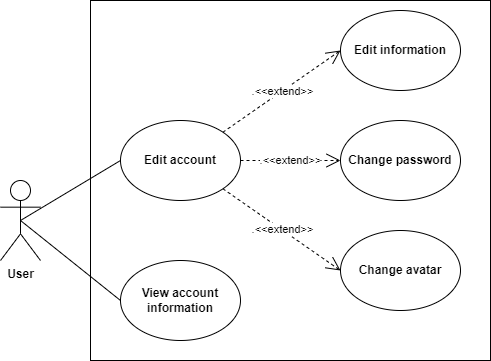
\includegraphics[width=0.8\textwidth]{Images/UseCase/Account.png}
    \caption{Sơ đồ use-case cho chức năng quản lý tài khoản}
\end{figure}
\subsubsection{Đặc tả use-case cho chức năng xem thông tin tài khoản}
\begin{center}
    \arrayrulecolor{cyan!75!black}
    \arrayrulewidth=2pt
    \begin{longtable}{
        |>{\raggedright\arraybackslash}p{3cm}
        |>{\raggedright\arraybackslash}p{13cm}
        |}
        \hline
        \rowcolor{cyan!75!black} \textcolor{white}{\textbf{Use-case name}} & \textcolor{white}{\textbf{XEM THÔNG TIN TÀI KHOẢN}}
        \\\hline
        \rowcolor{cyan!10!white} \textit{Actor} & Người dùng
        \\\hdashline
        \rowcolor{cyan!10!white} \textit{Description} & Tính năng cho phép người dùng xem thông tin cá nhân trên tài khoản của mình.
        \\\hdashline
        \rowcolor{cyan!10!white} \textit{Preconditions} & Người dùng đã đăng nhập vào tài khoản của mình.
        \\\hdashline
        \rowcolor{cyan!10!white} \textit{Postconditions} & Thông tin cá nhân của người dùng đã được hiển thị trên giao diện của ứng dụng.
        \\\hdashline
        \rowcolor{cyan!10!white} \textit{Trigger} & Người dùng chọn vào mục \textbf{Thông tin cá nhân} trên ứng dụng.
        \\\hdashline
        \rowcolor{cyan!10!white} \textit{Main flow} & 
        1. Ứng dụng hiển thị thông tin cá nhân trên giao diện. \newline
        2. Người dùng có thể theo dõi các thông tin cá nhân như tên, hình ảnh đại diện, email, số điện thoại, địa chỉ...
        \\\hdashline
        \rowcolor{cyan!10!white} \textit{Alternative flow} & Không có
        \\\hdashline
        \rowcolor{cyan!10!white} \textit{Exception flow} & 
        \textbf{Nếu ứng dụng gặp lỗi khi hiển thị thông tin tài khoản, ứng dụng thông báo lỗi và yêu cầu người dùng thử lại sau} \newline
        1a.1. Ứng dụng hiện lỗi khi hiển thị thông tin tài khoản. \newline
        1a.2. Ứng dụng thông báo yêu cầu người dùng thử lại sau.
        \\\hline
        \caption{Đặc tả use-case cho chức năng xem thông tin tài khoản}
    \end{longtable}
\end{center}
\subsubsection{Đặc tả use-case cho chức năng chỉnh sửa thông tin tài khoản}
\begin{center}
    \arrayrulecolor{cyan!75!black}
    \arrayrulewidth=2pt
    \begin{longtable}{
        |>{\raggedright\arraybackslash}p{3cm}
        |>{\raggedright\arraybackslash}p{13cm}
        |}
        \hline
        \rowcolor{cyan!75!black} \textcolor{white}{\textbf{Use-case name}} & \textcolor{white}{\textbf{CHỈNH SỬA THÔNG TIN TÀI KHOẢN}}
        \\\hline
        \rowcolor{cyan!10!white} \textit{Actor} & Người dùng
        \\\hdashline
        \rowcolor{cyan!10!white} \textit{Description} & Tính năng cho phép người dùng chỉnh sửa thông tin cá nhân trên tài khoản của mình.
        \\\hdashline
        \rowcolor{cyan!10!white} \textit{Preconditions} & Người dùng đã đăng nhập vào tài khoản của mình.
        \\\hdashline
        \rowcolor{cyan!10!white} \textit{Postconditions} & Thông tin cá nhân của người dùng đã được cập nhật thành công trên ứng dụng.
        \\\hdashline
        \rowcolor{cyan!10!white} \textit{Trigger} & Người dùng chọn \textbf{Chỉnh sửa} trong trang thông tin cá nhân.
        \\\hdashline
        \rowcolor{cyan!10!white} \textit{Main flow} &
        1. Ứng dụng hiển thị các trường thông tin cho phép chỉnh sửa trên giao diện ứng dụng. \newline
        2. Người dùng thực hiện việc chỉnh sửa thông tin cá nhân như tên, số điện thoại, địa chỉ... \newline
        3. Người dùng nhấn nút \textbf{Cập nhật} để cập nhật thông tin tài khoản. \newline
        4. Ứng dụng kiểm tra thông tin đã nhập và cập nhật vào dữ liệu. \newline
        5. Ứng dụng hiển thị thông báo cập nhật thành công.
        \\\hdashline
        \rowcolor{cyan!10!white} \textit{Alternative flow} &
        \textbf{Nếu người dùng không muốn thực hiện chỉnh sửa, họ có thể thoát ra khỏi giao diện chỉnh sửa thông tin người dùng} \newline
        2a.1. Người dùng nhấn nút \textbf{Hủy}. \newline
        2a.2. Ứng dụng chuyển hướng người dùng về trang thông tin cá nhân.
        \\\hdashline
        \rowcolor{cyan!10!white} \textit{Exception flow} &
        \textbf{Nếu thông tin cập nhật không hợp lệ, ứng dụng thông báo lỗi và yêu cầu người dùng cung cấp lại thông tin} \newline
        4a.1. Ứng dụng thông báo thông tin chỉnh sửa không hợp lệ. \newline
        4a.2. Người dùng nhập lại thông tin. \newline
        4a.3. Ứng dụng kiểm tra thông tin đã nhập. \newline
        4a.4. Nếu thông tin hợp lệ, ứng dụng sẽ thông báo chỉnh sửa thông tin tài khoản thành công, ngược lại sẽ quay lại bước 2. \newline
        \textbf{Nếu ứng dụng gặp lỗi khi xác minh thông tin tài khoản, ứng dụng thông báo lỗi và yêu cầu người dùng thử lại sau} \newline
        4b.1. Ứng dụng hiện lỗi khi xác minh thông tin tài khoản. \newline
        4b.2. Ứng dụng thông báo yêu cầu người dùng thử lại sau.
        \\\hline
        \caption{Đặc tả use-case cho chức năng chỉnh sửa thông tin tài khoản}
    \end{longtable}
\end{center}
\subsubsection{Đặc tả use-case cho chức năng đổi mật khẩu}
\begin{center}
    \arrayrulecolor{cyan!75!black}
    \arrayrulewidth=2pt
    \begin{longtable}{
        |>{\raggedright\arraybackslash}p{3cm}
        |>{\raggedright\arraybackslash}p{13cm}
        |}
        \hline
        \rowcolor{cyan!75!black} \textcolor{white}{\textbf{Use-case name}} & \textcolor{white}{\textbf{ĐỔI MẬT KHẨU}}
        \\\hline
        \rowcolor{cyan!10!white} \textit{Actor} & Người dùng
        \\\hdashline
        \rowcolor{cyan!10!white} \textit{Description} & Tính năng cho phép người dùng đổi mật khẩu cho tài khoản của mình.
        \\\hdashline
        \rowcolor{cyan!10!white} \textit{Preconditions} & Người dùng đã đăng nhập vào tài khoản của mình.
        \\\hdashline
        \rowcolor{cyan!10!white} \textit{Postconditions} & Mật khẩu của người dùng đã thay đổi thành công trên ứng dụng.
        \\\hdashline
        \rowcolor{cyan!10!white} \textit{Trigger} & Người dùng chọn \textbf{Đổi mật khẩu} trong trang thông tin cá nhân.
        \\\hdashline
        \rowcolor{cyan!10!white} \textit{Main flow} &
        1. Ứng dụng hiển thị các trường thông tin cho phép cập nhật mật khẩu trên giao diện ứng dụng. \newline
        2. Người dùng cung cấp mật khẩu hiện tại và mật khẩu muốn đổi. \newline
        3. Người dùng nhấn nút \textbf{Cập nhật} để cập nhật mật khẩu. \newline
        4. Ứng dụng kiểm tra thông tin đã nhập và cập nhật vào dữ liệu. \newline
        5. Ứng dụng hiển thị thông báo cập nhật mật khẩu mới thành công.
        \\\hdashline
        \rowcolor{cyan!10!white} \textit{Alternative flow} &
        \textbf{Nếu người dùng không muốn thực hiện đổi mật khẩu, họ có thể thoát ra khỏi giao diện chỉnh sửa thông tin người dùng} \newline
        2a.1. Người dùng nhấn nút \textbf{Hủy}. \newline
        2a.2. Ứng dụng chuyển hướng người dùng về trang thông tin cá nhân.
        \\\hdashline
        \rowcolor{cyan!10!white} \textit{Exception flow} &
        \textbf{Nếu người dùng không cung cấp thông tin mật khẩu hiện tại hoặc mật khẩu mới, ứng dụng thông báo lỗi và yêu cầu người dùng cung cấp đầy đủ thông tin} \newline
        4a.1. Ứng dụng thông báo thông tin còn bị thiếu sót. \newline
        4a.2. Người dùng cập nhật đầy đủ. \newline
        4a.3. Ứng dụng kiểm tra thông tin đã nhập. \newline
        4a.4. Nếu thông tin hợp lệ, ứng dụng sẽ thông báo cập nhật mật khẩu cho thành công, ngược lại sẽ quay lại bước 2. \newline
        \textbf{Nếu mật khẩu hiện tại không khớp, ứng dụng thông báo lỗi và yêu cầu người dùng cung cấp lại mật khẩu hiện tại} \newline
        4b.1. Ứng dụng thông báo mật khẩu hiện tại không khớp. \newline
        4b.2. Người dùng nhập lại mật khẩu hiện tại. \newline
        4b.3. Ứng dụng kiểm tra thông tin đã nhập. \newline
        4b.4. Nếu thông tin hợp lệ, ứng dụng sẽ thông báo cập nhật mật khẩu cho tài khoản thành công, ngược lại sẽ quay lại bước 2. \newline
        \textbf{Nếu ứng dụng gặp lỗi khi cập nhật mật khẩu, ứng dụng thông báo lỗi và yêu cầu người dùng thử lại sau} \newline
        4c.1. Ứng dụng hiện lỗi khi cập nhật mật khẩu. \newline
        4c.2. Ứng dụng thông báo yêu cầu người dùng thử lại sau.
        \\\hline
        \caption{Đặc tả use-case cho chức năng đổi mật khẩu}
    \end{longtable}
\end{center}
